\documentclass[12pt]{article}
\usepackage[utf8]{inputenc}

\newenvironment{sol}[1][Solution]{\begin{trivlist}\item[\hskip\labelsep {\bfseries #1:}]}{\end{trivlist}}
\usepackage[margin=1in]{geometry} 
\usepackage{amsmath,amsthm,amssymb}
\usepackage{minted}
\usemintedstyle{vs}
\usepackage{graphicx}
\graphicspath{{./images}}
\usepackage{ amssymb }

\title{Southern Methodist University \\
Bobby B. Lyle School of Engineering Department of Computer Science \\
Homework 2
}

\author{Operating System and Software System \\
Name: Bingying Liang 
\\ ID: 48999397\\ 
Email: bingyingl@smu.edu \\ 
CS7343 Distance}
\date{February 2 2023}

\begin{document}

\maketitle

\begin{itemize}
    \item Include a front page with course title, your name, Student ID, your e-mail address, and the course number (e.g. CS 5343 or CS 7343). You must also indicate whether you are a distance student or an in-person student.

    \item Each answer should begin in a new page.
    \item \textcolor{red}{Note:}
    \begin{itemize}
        \item[$\bullet$] There will be 10 points deduction if this information is missing.
        \item[$\bullet$] Late Homework submission must be sent directly to the grader via email.
        \textcolor{red}{\item[$\bullet$] All students who are signed for this course at the CS 7343 must answer all questions.
        \item[$\bullet$]  All students who are signed for this course at the CS 5343 must answer exactly four questions.}
    \end{itemize}

\end{itemize}
\newpage
\begin{enumerate}
    \item Consider the following program:
 \begin{minted}[frame=lines,framesep=2mm,baselinestretch=1.2,fontsize=\footnotesize]{c}
const int n = 50;
int tally;
void total()
{
    int count;
    for (count = 1; count <= n; count++){
        tally++;
    }
}

void main()
{
    tally = 0;
    Parbegin (total (), total ());
    write (tally);
}
\end{minted}
The key word Parbegin indicates that both calls to the function total are executed concurrently. Determine the proper lower bound and upper bound on the final value of the shared variable tally output by this concurrent program. Assume processes can execute at any relative speed and that a value can only be incremented after it has been loaded into a register by a separate machine instruction. You must explain how you’ve arrived to the final answer.
\begin{sol}
\hspace*{\fill}\\
1) tally is the only shared valuable.\\
2) The constant n is read only and its thread safe.\\
3) The valuable count is local to the function total() and hence each thread has its own copy of the valuable count.\\
4) The statement $tally$\texttt{++} is the one that must addressed. Because $tally$\texttt{++} $ \rightarrow tally = tally +1;$ and $tally$ is shared valuable and is accessible by both threads.\\
\\
Upper bound on the final value of the shared variable $tally$ is 100.\\
\textbf{Explain:} Because the Parbegin indicates that both calls to the function total are executed concurrently which means we have two threads. And when threads run in sequenced manner will have the upper bound. The one of $total()$ thread can finished firstly. During the situation the $tally = 50$ and then another then keep finish and it will start from $tally = 50, count = 0, n = 50 $  and then it finishes the result of the $tally$ will be 100.   

Lower bound on the final value of the shared variable $tally$ is 2.\\
\textbf{Explain: } $tally + 1 = tally$ transfer to assembly language(e.g MIPS) will be 
\begin{minted}[frame=lines,framesep=2mm,baselinestretch=1.2,fontsize=\footnotesize]{c}
(1) lw R0, tally
(2) add R0, 1
(3) sw R0, tally 
\end{minted}
And can treat the first $total()$ as Thread A, and the second $total()$ as Thread B. And the process in the following:\\
\textbf{A:} $tally = 0, R_0 = 0 $ \\ 
$ (1) R_0 = 0 \ (2) R_0 = 1 \ ... \ suspend \ (3) \ $ \\ 
$n = 1$  (The thread A (3) has not finished yet. The thread turns to B)\\
\\
\textbf{B:} $tally = 0, R_0=0$ \\
$ (1) R_0 = 0 \ (2) R_0 = 1 \ (3) tally = R_0 = 1 \dots \ (1) R_0 = 48 \ (2) R_0 = 49 \ (3) tally = 49$ \\ 
$n = 49$  (The thread turns to A)\\
\\
\textbf{A:} $tally = 49, R_0 = 1$\\
$ (3) sw \ R_0, tally \rightarrow tally = 1$\\
$n = 1$ (The thread turns to B)\\
\\
\textbf{B:} $tally = 1, R_0 = 0$\\
$(1) R_0 = 1 \ (2) R_0 = 2 \ suspend\ (3) $\\
$n = 50$ (The thread B (3) has not finished yet. The thread turns to A)\\
\\
\textbf{A:} $tally = 1, R_0 = 0$\\
$(1) R_0 = 1 \ (2) R_0 = 2 \ (3) tally = R_0 = 2 \dots (1)R_0 = 49\ (2) R_0 = 50 \ (3)tally = R_0 = 50$\\
$n = 50$ (The thread A has finished. The thread turns to B)\\
\\
\textbf{B:} $tally = 50, R_0 = 2$\\
$(3) tally = R_0 = 2$\\
$n = 50$ (The thread B has finished. The $tally$ is equal to $2$).

\end{sol}
\textcolor{red}{Hints: Notice that we have two threads (call them T1 and T2) running simultaneously. This is evident from the two concurrent invocation of the function total() two times. Also, notice that the variable tally is shared. This implies that both threads have access to the same variable and, hence, they may modify the value of tally independent of each other.\\
Under the best scenario, both T1 and T2 will run sequentially. In this case, T1 will run into completion followed by T2 as in }
 \begin{minted}[frame=lines,framesep=2mm,baselinestretch=1.2,fontsize=\footnotesize]{c}
void main()
{
    tally = 0;
    total (); 
    total ();
}
\end{minted}
\textcolor{red}{On the other hand, Thread T1 and T2 could be running in such a way so that they will Tally++\\
Assembly: In this assembly code tally is a location in memory and R0 of the CPU registers}
 \begin{minted}[frame=lines,framesep=2mm,baselinestretch=1.2,fontsize=\footnotesize]{c}
1. load tally to R0
2. increment R0
3. move R0 to tally
\end{minted}
\textcolor{red}{Consider the following scenario
\begin{enumerate}
    \item[(1)] Thread A loads the value of tally, increments tally, but then loses the processor(it has incremented its register to 1, but has not yet stored this value.)
    \item[(2)] Thread B loads the value of tally (still zero) and performs forty-nine complete increment operations, losing the processor after it has stored the value 49 into the shared variable tally.
    \item[(3)] Thread A regains control long enough to perform its first store operation(replacing the previous tally value of 49 with 1) but is then immediately forced to relinquish the processor.\\
    There are three execution steps that Thread A and Thread B could execute that result in the minimum value of tally. Try to deduce these steps.
    \item[(4)] Thread B resumes long enough to load 1 (the current value of tally) into its register, but then it too is forced to give up the processor (note that this will B's final load).
    \item[(5)] Thread A is rescheduled, but this time it is not interrupted and runs to completion, performing its remaining 49 load, increment, and store operations, which results in setting the value of tally to 50.
    \item[(6)] Thread B is reactivated with only one increment and store operation to perform before it terminates. It increments its register value to 2 and stores this value as the final value of the shared variable.
\end{enumerate}
}
\newpage
\item Examine the following pseudo code in which p and q, defined as shown below. A, B, C, D, and E atomic (indivisible) statements. Assume that the main program execute these two processes concurrently.
 \begin{minted}[frame=lines,framesep=2mm,baselinestretch=1.2,fontsize=\footnotesize]{c}
void p()                   void q()
{                          {
    A;                          D;
    B;                          E;
    C;                      }
}

void main()
{
    Parbegin p(),q() // Call method p() and method q() simultaneously
}
\end{minted}
\begin{enumerate}
    \item Show all possible execution paths of this program. For example, a possible execution path would be ABCDE.
    \item Show 5 paths of this program. For example, an impossible path would be EDABC.
\end{enumerate}
\begin{sol}
\hspace*{\fill} 
\begin{enumerate}
\item There are 10 possible execution paths of this program.
\begin{enumerate}
    \item ADEBC
    \item ADBEC
    \item ADBCE
    \item ABDEC
    \item ABDCE
    \item ABCDE
    \item DEABC
    \item DAEBC
    \item DABEC
    \item DABCE
    
\end{enumerate}
\item Impossible paths are: 
$$all \ paths - possible \ execution \ paths = 5! - 10 = 120 - 10 = 110$$
And they are Bxxxx, Exxxx, Cxxxx, AExxx, ACxxx, DBxxx, DCxxx, ABExx, ADCxx, DACxx, DEBxx, DECxx, ABCEx, ADECx, DEACx, DAECx (x are the remain statements).\\ Show 5 paths of impossible paths are: AEBCD, AEBDC, AECBD, AECDB, AEDBC.
\end{enumerate}

\end{sol}
\textcolor{red}{Hints: The easiest way is to graphically show all possible paths and subtract from them the legal pahts stated in part a. Or simply all paths except those in part a are impossible.}

\newpage
\item For each of the following thread state transitions, say whether the transition is legal and how the transition occurs or why it cannot.
\begin{enumerate}
    \item Change from thread state BLOCKED to thread state RUNNING
    \item Change from thread state RUNNING to thread state BLOCKED
    \item Change from thread state RUNNABLE (i.e., in the ready queue) to thread state BLOCKED
\end{enumerate}
\begin{sol}
    ~\
    \begin{enumerate}
        \item The transition is illegal.\\
        Because before the RUNNING state, the thread should be waiting to be assigned to a processor in the READY state. And then it waiting a turn to run on CPU which is RUNNING state.
        \item The transition is legal.\\
        Because during the execution of the thread, the thread might require some I/O operation like writing on file or some more priority thread might come. In these situations, the running thread will have to go into the blocked or waiting state and the other thread will come for its execution. 
        \item The transition is illegal.\\
        Because the thread has already in the ready queue, which is generally stored as a linked list and a ready-queue header contains pointer to the first in the list. The thread will execute in order into RUNNING state and then it can change to BLOCKED state.
    \end{enumerate}
\end{sol}
\textcolor{red}{Hints:
\begin{enumerate}
    \item[(a)] Illegal. The scheduler selects threads to run from the list of ready (or runnable) threads. A blocked thread must first be placed in the ready queue before it can be selected to run. 
    \item[(b)] Legal. A running thread can become blocked when it requests a resource that is not immediately available (disk I/O, lock etc).
    \item[(c)] Illegal. A thread can only transition to BLOCKED from RUNNING. It cannot execute any statements when still in a queue (i.e. the ready queue).
\end{enumerate}}

\newpage
\item Consider an environment in which there is an equivalence mapping between user-level and kernel-level threads (i.e. that is we have a one-to-one mapping between user threads and kernel threads) that allows one or more threads within a process to issue blocking system calls while other threads continue to run. Will this approach make multithreaded programs run faster than their single-threaded counterparts on a uniprocessor computer?
\begin{sol}
\hspace*{\fill} \\
This approach will make multithreaded programs run faster than their single-threaded counterparts on uniprocessor computer. Because it provides more concurrency by allowing another thread to run when a thread makes a blocking system call. It also allows multiple threads to run in parallel on multiprocessors. And also in this type of system, the blocking system cannot block the complete execution because kernel thread is present for every user thread. So, if one kernel thread gets blocked, others will still keep running. \\
\\
There are four main reasons and benefits: \\
(1) First, Responsiveness. Multithreading an interactive application may allow a program to continue running even if part of it is blocked or is performing a lengthy operation, thereby increasing responsiveness to the user. \\
\\
(2) Second, Resource sharing. Processes can share resources only through techniques such as shared memory and message passing. \\
\\
(3) Third, Economy. Allocating memory and resources for process creation is costly. Because threads share the resources of the process to which they belong, it is more economical to create and context-switch threads.\\
\\
(4) Fourth, Scalability. The benefits of multithreading can be even greater in a multiprocessor architecture, where threads may be running in parallel on different processing cores.\\

\end{sol}
\textcolor{red}{Hints: The issue here is that a machine spends a considerable amount of its waking hours waiting for I/O to complete. In a multithreaded program, one KLT can make the blocking system call, while the other KLTs can continue to run. On uniprocessors, a process that would otherwise have to block for all these calls can continue to run its other threads.}

\newpage
\item Consider the figure below. Show all possible transitions and give a scenario in which each transition could occur.\\
    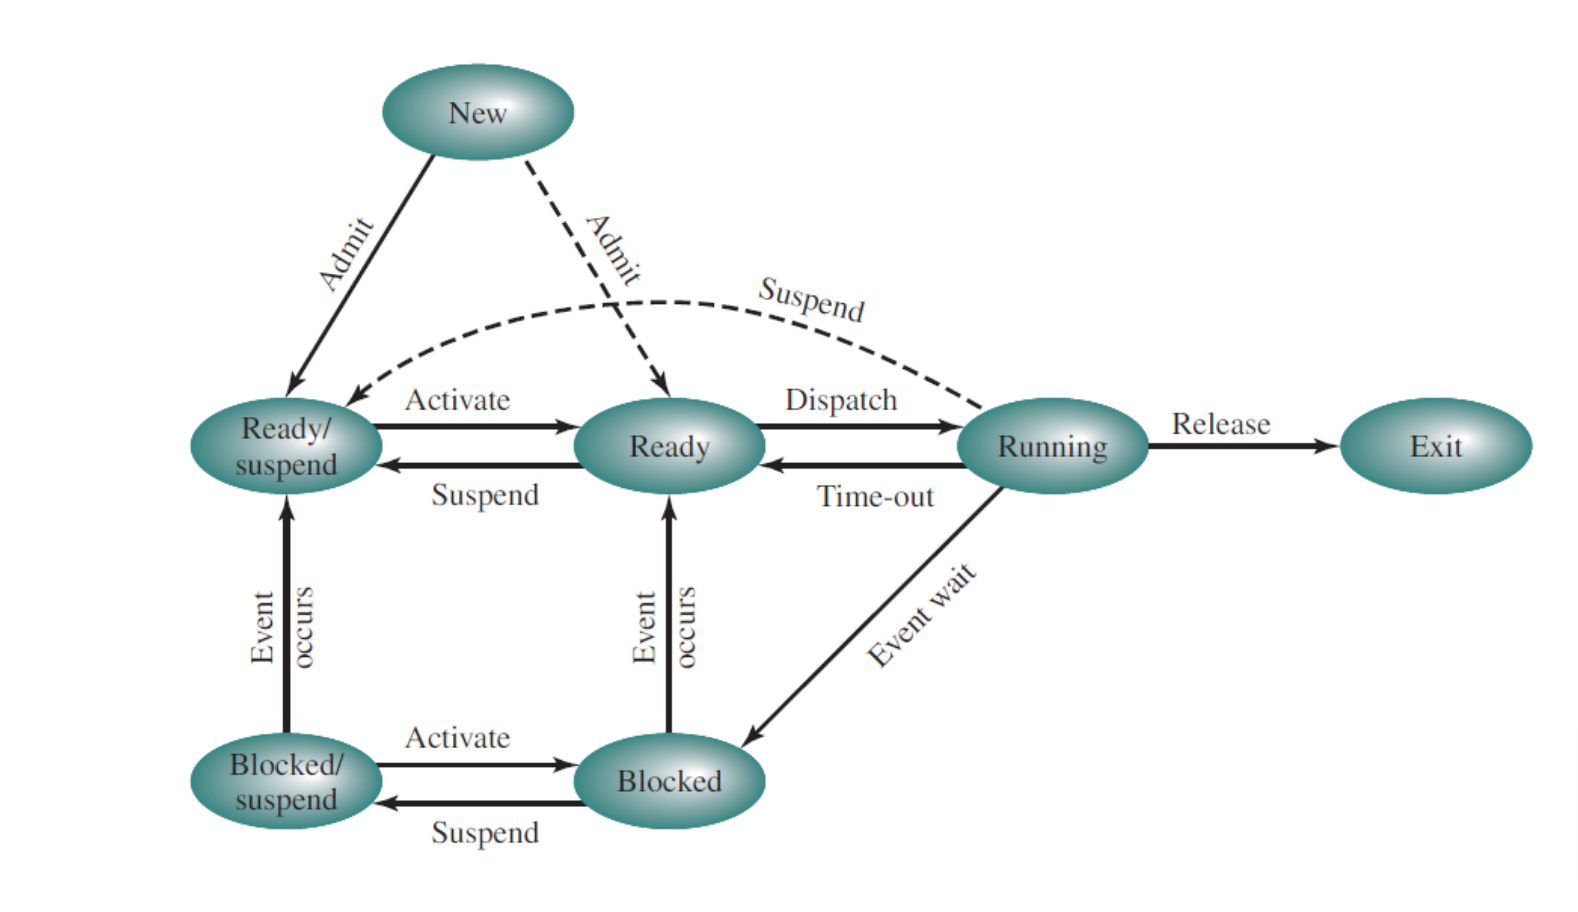
\includegraphics[width=0.9\textwidth]{problem5.png}
\begin{sol}
\hspace*{\fill} \\
State definitions:\\
New: In this step, the process is about to be created but not yet created, it is the program which is present in secondary memory that will be picked up by OS to create the process.\\
Ready: The process is in main memory and available for execution. It does not have a possession of the processor yet. In other words, it is ready but waiting on a turn to run on the CPU.\\
Running: The process is chosen by CPU for execution and the instructions within the process are executed by any one of the available CPU cores.\\
Blocked: The process is in main memory and waiting for an event. (e.g. I/O process)\\
Blocked/suspend: The process is in disk and awaiting an event.\\
Ready/suspend: The process is in disk, but available for execution as soon as it is loaded into main memory.\\
In terms of who/which state is closest to be running under normal circumstances:\\
1) Running state \\
2) Ready \\
3) Blocked \\
4) Ready/suspend \\
5) Blocked/suspend \\

\begin{enumerate}
    \item $New \xrightarrow[]{Admit} Ready/suspend$\\
    There can be more than one process in the ready state but due to memory constraint, if the memory is full then some process from the ready state gets placed in the ready suspended state. For example, open a lot of applications on a laptop, and at the same time the memory is full the new process will be into Ready/suspend state.
    \item $New \xrightarrow[]{Admit}  Ready$\\
    For example, create new process like calculate $x=2, y= 3, w = x + y?$ , should load the $x, y$ to the register first and then wait in the ready queue to get its turn of running in the CPU. And another example is a user opens up a word processor, once the process has completed its initialization it is placed in a Ready state with all of the other processes waiting to take its turn on the CPU. 
    \item $Ready \xrightarrow[]{Suspend} Ready/suspend$ \\
    Whenever the main memory is full, the process which is in a ready state is swapped out from main memory to secondary memory. For example, a laptop are running process, and then its main memory is full. It will let some ready state like low priority process change to the Ready/suspend state. Once the main memory will have enough space for the process, the process will be brought back to the main memory and will be in a ready state.
    \item $Ready \xrightarrow[]{Dispatch} Running$\\
    For example, when the process of $x=2, y= 3, w = x + y?$ are the ready state and the ready queue pointers turn to it which means the it's its turn to run on the CPU it will become Running state.
    \item $Running \xrightarrow[]{Time-out} Ready$\\
    The process uses up it turn but for some reason it's Timeout and then is returned to the Ready state. For example, it we running some process or programs, it costs too long, the OS will jump out some windows to alarm user to try again or do another instructions. Another situation is about the priority. A transition from Running state to Ready state can happen only in case the OS uses a preemptive scheduler. Some examples of preemptive scheduling algorithms are Round Robin Scheduling Algorithm or Preemptive Priority Based Scheduling Algorithm and so on, these algorithms the scheduler can select another process to RUN, while some process is already running on the Processor. In such a situation the Running process is said to be "PREEMPTED" and moved from Running state to Ready queue.
    
    \item $Running \xrightarrow[]{Release} Exit$\\
        When the entire set of instructions is executed and the process is completed. The process is changed to terminated or completed state. For example, CPU has ready finishes the $x=2, y= 3, w = x + y = 5$ and return and store the w back. The process is Exit. Or we we open the application and turn if off. The Running process exit. 
    \item $Running \xrightarrow[]{Event \ wait} Blocked$\\
        A process change from Running state to a blocked state when it cannot carry on without an external change in state or event occurring. For example, a process may block on a call to an I/O device such as a printer, if the printer is not available. Processes also commonly block when they require user input, or require access to a critical section which must be executed atomically. 
    \item $Running \xrightarrow[]{Suspend} Ready/suspend$\\
        The process is timeout and OS should reschedule it, but at the same time, the memory of computer is full, and then the process will change Running state into Ready/suspend until the main memory has enough space for the process. And in another situation like running the process the OS find some deadlocks or something like that and the main memory does not have enough space, the process will also change the Running state into Ready/suspend state.
    \item $Blocked \xrightarrow[]{Event \ occur} Ready$\\
        Whenever the process requests access to I/O or needs input from the user or needs access to a critical region(the lock for which is already acquired) it enters the blocked or wait state. The process continues to wait in the main memory and does not require CPU. Once the I/O operation is completed the process goes to the ready state. For example, when the user finishes input by keyboard or something else, it will change the Blocked state to the Ready state.
    \item $Blocked \xrightarrow[]{Suspend} Blocked/suspend$\\
    Similar to suspend ready but uses the process which was performing I/O operation and lack of main memory caused them to move to secondary memory. For example, the memory of laptop is full, waiting user to input something it will no have the space, it will let the process like lower priority change into Blocked/suspend state until has the memory let user input something. Or for a long time user does not input something it will also change the state.
    \item $Blocked/suspend \xrightarrow[]{Activate} Blocked$\\
    For example, when the user has enough memory for the process and then user can input something from keyboard, and then it will change the state from Blocked/suspend state Blocked state, let user input something to keep the process to the next step. 
    \item $Blocked/suspend \xrightarrow[]{Event \ occur} Ready/suspend$\\
    For example, now do not have enough memory or for a long time waiting user to input something from keyboard and then user has done it. The process will change the Blocked/suspend into Ready/suspend waiting for transfer data from secondary memory into main memory.
    \item $Ready/suspend \xrightarrow[]{Activate} Ready$\\
    When the computer has enough memory allow the data from secondary memory into the main memory, it will allow the process state of Ready/suspend change to Ready state. For example, process like calculate $x=2, y= 3, w = x + y?$ has enough memory to load  $x, y$ to the register first and then wait in the ready queue to get its turn of running in the CPU.
    
    
\end{enumerate}

\end{sol}
\textcolor{red}{Hints: 
\begin{enumerate}
    \item \textbf{New $\rightarrow$ Ready or Ready/Suspend:} When a new process is created, it can either be added to the Ready queue or the Ready/Suspend queue. In either case, the OS must create a process control block and allocate an address space to the process. It might be preferable for the OS to perform these housekeeping duties at an early time, so that it can maintain a large pool of processes that are not blocked. With this strategy, there would often be insufficient room in main memory for a new process; hence the use of the (New$\rightarrow$ Ready/Suspend) transition. On the other hand, we could argue that a just-in-time philosophy of creating processes as late as possible reduces OS overhead and allows that OS to perform the process-creation duties at a time when the system is clogged with blocked processes anyway.\\
    \textbf{Ready $\rightarrow$ Running:} When it is time to select a process to run, the OS chooses one of the processes in the Ready state. This is the job of the scheduler or dispatcher. 
    \textbf{Ready $\rightarrow$ Ready/Suspend:} Normally, the OS would prefer to suspend a blocked process rather than a ready one, because the ready process can now be executed, whereas the blocked process is taking up main memory space and cannot be executed. However, it may be necessary to suspend a ready process if that is the only way to free up a sufficiently large block of main memory. Also, the OS may choose to suspend a lower-priority ready process rather than a higher-priority blocked process if it believes that the blocked process will be ready soon. \\
    \textbf{Ready/Suspend$\rightarrow$ Ready:} When there are no ready processes in main memory, the OS will need to bring one in to continue execution. In addition, it might be the case that a process in the Ready/Suspend state has higher priority than any of the processes in the Ready state. In that case, the OS designer may dictate that it is more important to get at the higher-priority process than to minimize swapping.\\
    \textbf{Blocked $\rightarrow$ Ready:} A process in the Blocked state is moved to the Ready state when the event for which it has been waiting occurs.\\
    \textbf{Blocked $\rightarrow$ Blocked/Suspend: }If there are no ready processes,then at least one blocked process is swapped out to make room for another process that is not blocked. This transition can be made even if there are ready processes available, if the OS determines that the currently running process or a ready process that it would like to dispatch requires more main memory to maintain adequate performance.\\ 
    \textbf{Blocked/suspend $\rightarrow$ Ready/Suspend:} A process in the Blocked/Suspend state is moved to the Ready/Suspend state when the event for which it has been waiting occurs. Note that this requires that the state information concerning suspended processes must be accessible to the OS.\\
    \textbf{Blocked/suspend $\rightarrow$ Blocked:} Inclusion of this transition may seem to be poor design. After all, if a process is not ready to execute and is not already in main memory, what is the point of bringing it in? But consider the following scenario: A process terminates, freeing up some main memory. There is a process in the (Blocked/Suspend) queue with a higher priority than any of the processes in the (Ready/Suspend) queue and the OS has reason to believe that the blocking event for that process will occur soon. Under these circumstances, it would seem reasonable to bring a blocked process into main memory in preference to a ready process.\\
    \textbf{Running $\rightarrow$ Ready:} The most common reason for this transition is that the running process has reached the maximum allowable time for uninterrupted execution; virtually all multiprogramming operating systems impose this type of time discipline. There are several other alternative causes for this transition, which are not implemented in all operating systems. Of particular importance is the case in which the OS assigns different levels of priority to different processes. Suppose, for example, that process A is running at a given priority level, and process B, at a higher priority level, is blocked. If the OS learns that the event upon which process B has been waiting has occurred, moving B to a ready state, then it can interrupt process A and dispatch process B. We say that the OS has preempted process A. Finally, a process may voluntarily release control of the processor. An example is a background process that performs some accounting or maintenance function periodically.\\
    \textbf{Running $\rightarrow$ Ready/suspend:} Normally, a running process is moved to the Ready state when its time allocation expires. If, however, the OS is preempting the process because a higher-priority process on the Blocked/Suspend queue has just become unblocked, the OS could move the running process directly to the (Ready/Suspend) queue and free some main memory.\\
    \textbf{Running $\rightarrow$ Blocked:} A process is put in the Blocked state if it requests some- thing for which it must wait. A request to the OS is usually in the form of a system service call; that is, a call from the running program to a procedure that is part of the operating system code. For example, a process may request a service from the OS that the OS is not prepared to perform immediately. It can request a resource, such as a file or a shared section of virtual memory, that is not immediately available. Or the process may initiate an action, such as an I/O operation, that must be completed before the process can continue. When processes communicate with each other, a process may be blocked when it is waiting for another process to provide data or waiting for a message from another process.\\
    \textbf{Any State $\rightarrow$ Exit: }Typically, a process terminates while it is running, either because it has completed or because of some fatal fault condition. However, in some operating systems, a process may be terminated by the process that created it or when the parent process is itself terminated. If this is allowed, then a process in any state can be moved to the Exit state.
    \item \textbf{New $\rightarrow$ Blocked, Blocked/Suspend, or Running:} A newly created process remains in the new state until the processor is ready to take an additional process, at which time it goes to one of the Ready states.\\
    \textbf{Ready $\rightarrow$ Blocked or Blocked/Suspend:} Typically, a process that is ready cannot subsequently be blocked until it has run. Some systems may allow the OS to block a process that is currently ready, perhaps to free up resources committed to the ready process.\\
    \textbf{Ready/suspend $\rightarrow$ Blocked or Blocked/Suspend:} Same reasoning as preceding entry.\\
    \textbf{Ready/Suspend $\rightarrow$ running: }The OS first brings the process into memory, which puts it into the Ready state.\\
    \textbf{Blocked $\rightarrow$ Ready/Suspend:} this transition would be done in 2 stages. A blocked process cannot at the same time be made ready and suspended, because these transitions are triggered by two different causes.\\
   \textbf{ Blocked $\rightarrow$ Running:} When a process is unblocked, it is put into the Ready state. The dispatcher will only choose a process from the Ready state to run. \\
    \textbf{Blocked/Suspend $\rightarrow$ Ready: }same reasoning as Blocked $\rightarrow$ Ready/Suspend\\
    \textbf{Blocked/Suspend $Running$:} same reasoning as Blocked $\rightarrow$ Running.
    \textbf{Running $\rightarrow$ Blocked/Suspend:} this transition would be done in 2 stages \\
    \textbf{Exit $\rightarrow$ Any State:} Can't turn back the clock.
\end{enumerate}
}

\newpage
\item Consider the Shell sort algorithm as explained in \\
https://www.youtube.com/watch?v=ddeLSDsYVp8 \\
Is it possible to use two or more threads to implement this algorithm. Explain why/why not.
\begin{sol}
Yes, it is possible to use two or more threads to implement this algorithm.
\textbf{Explain:} Shell sort algorithms begins by performing a gap insertion sort, with the gap being the first number in the increment sequence. It continues to perform a gap insertion sort for each number in the sequence, until it finishes with a gap of 1. When the increment reaches 1, the gap insertion sort is simply an ordinary insertion sort, guaranteeing that the final list is sorted. Beginning with large increments allows elements in the file to move quickly towards their final positions, and makes it easier to subsequently sort for smaller increments. \\
Above are the definition of the shell sort. During the beginning, for example an array are divide by gap into different parts and than swap them. We can tread the different parts as thread and swap them in the concurrency. \\
Take $array = [7, 6, 8, 9, 3, 2, 10, 5, 1]$ for example:\\
(1) $gap = 3$ \\
    \begin{equation*}
    \begin{matrix}
    & 7 & 6 & 8 & 9 & 3 & 2 & 10 & 5 & 1\\
Thread_1& 7 &   &   &   & 3 &   &    &   &   \\
Thread_2& & 6 &   &   &   & 2 &    &   &   \\
Thread_3& &   & 8 &   &   &   & 10  &   &   \\
Thread_4& &   &   & 9 &   &   &    & 5  &   \\
Thread_5& &   &   &   &   &   &    &   &  1 \\
    \end{matrix}
    \end{equation*}
Finishing the threads of swapping it will become 
    \begin{equation*}
        \begin{matrix}
            

    & 7 & 6 & 8 & 9 & 3 & 2 & 10 & 5 & 1\\
Thread_1& 3 &   &   &   & 7 &   &    &   &   \\
Thread_2& & 2 &   &   &   & 6 &    &   &   \\
Thread_3& &   & 8 &   &   &   & 10  &   &   \\
Thread_4& &   &   & 5 &   &   &    & 9  &   \\
Thread_5& &   &   &   &   &   &    &   &  1 \\
Array & 3&2   & 8  & 5  & 7  & 6  & 10   &9   &  1 \\
        \end{matrix}
    \end{equation*}

(2) $gap = 2$ ... \\
(3) $gap = 1$ ...\\
(3) $gap = 0$ do insertion sort. And then $result = [1, 2, 3, 5, 6, 7, 8, 9, 10]$ \\
Therefore, it is possible to use two or more threads to implement this algorithm.


\end{sol}
\textcolor{red}{Hints: Yes. Each subset of the unsorted list can be independently sorted by a separate thread.}

\newpage
\item Suppose a process P spawns one or more threads. If the process P terminates and exits, will these threads continue to run? Explain.
\begin{sol}
\hspace*{\fill} \\
If the process P terminates and exits, these threads will not continue to run. \\
Because all threads in a process share the same address space, all threads are suspended at the same time. Similarly, termination of a process terminates all threads within that process.\\
For example:\\
    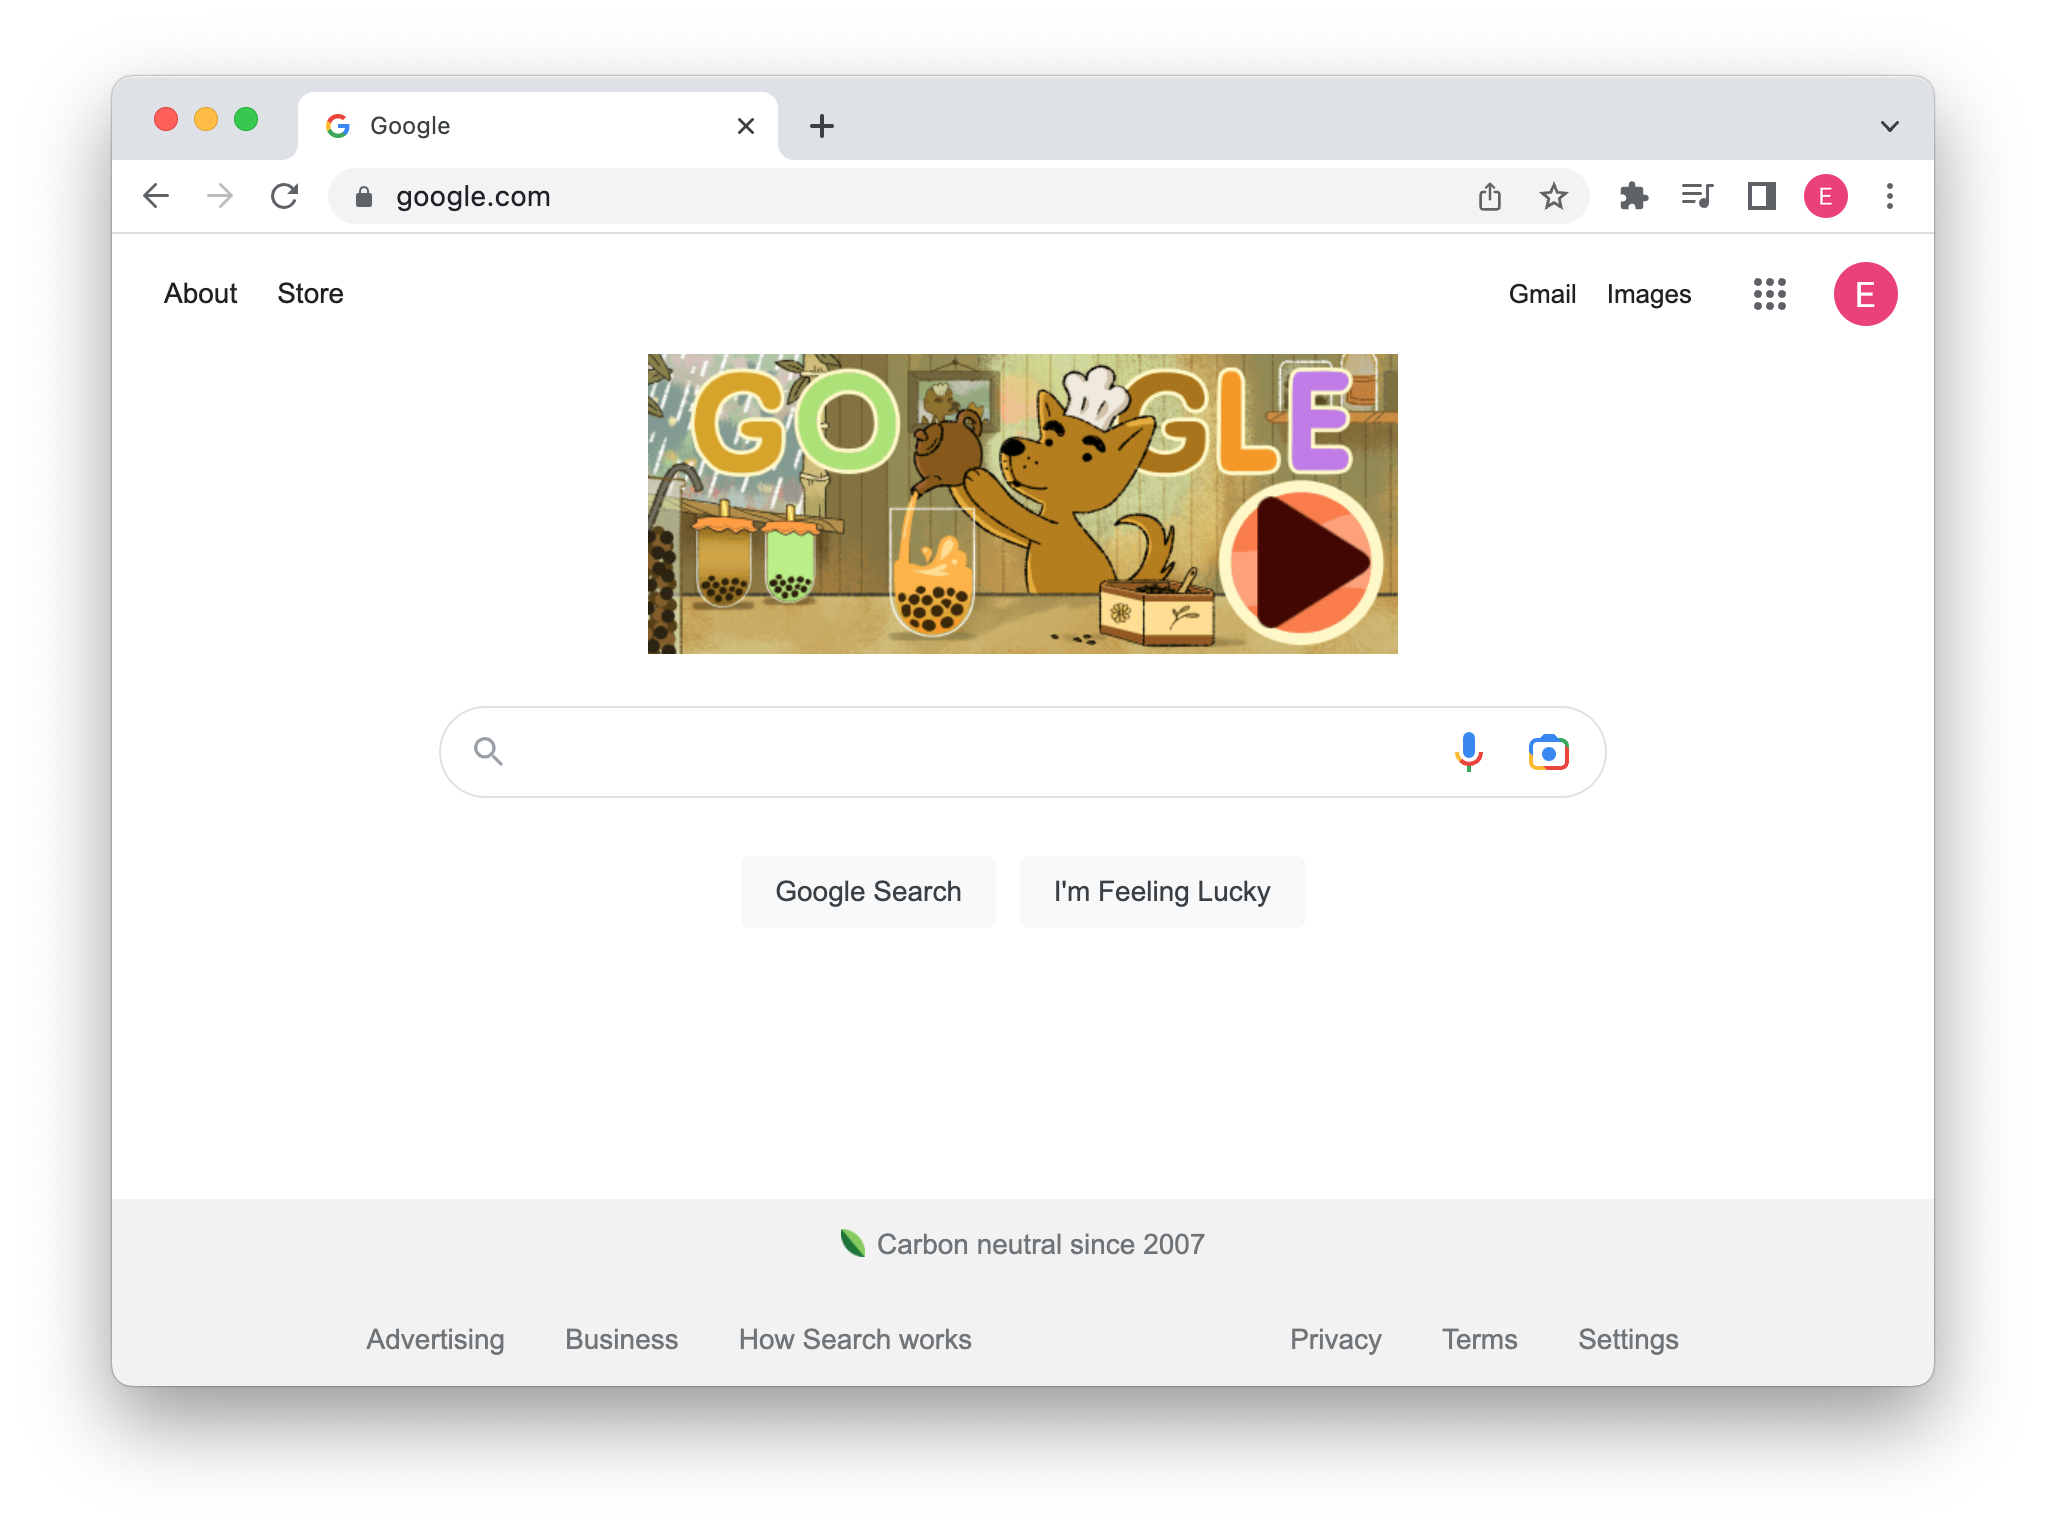
\includegraphics[width=0.9\textwidth]{problem7.png}\\
    When user open the Chrome, the process has been created. And then click add new tab here, the user is creating thread right here. \\
    
\includegraphics[width=0.9\textwidth]{problem7b.png}\\
    User can kill one thread(remove one tab at a time), the process are not terminates. However, if user exit or click the close button of the Chrome.\\
    \begin{center}
        
\includegraphics[width=0.08\textwidth]{problem7c.png}
    \end{center}
    All the threads (tab) can not run any more.
    
    
\end{sol}
\textcolor{red}{Hints: No. When a process exit, it takes everything with it -- the KLTS, the process structure, the memory space, everything -- including threads.}

\end{enumerate}



\end{document}
